\documentclass{report}
\usepackage[T1]{fontenc} % Fontes T1
\usepackage[utf8]{inputenc} % Input UTF8
\usepackage[backend=biber, style=ieee]{biblatex} % para usar bibliografia
\usepackage{csquotes}
\usepackage[portuguese]{babel} %Usar língua portuguesa
\usepackage{blindtext} % Gerar texto automaticamente
\usepackage[printonlyused]{acronym}
\usepackage{hyperref} % para autoref
\usepackage{graphicx}
\usepackage{subfig}
\usepackage{indentfirst}
\usepackage{amsmath}
\usepackage{xfrac}
\usepackage{mathtools}
\usepackage{wrapfig} %imagem no meio do texto
\bibliography{bibliografia} % para indicar que o ficheiro de bibliografia é o bibliografia.bib

\begin{document}
%%
% Definições
%
\def\titulo{Inteligência Artificial}
\def\data{DATA}
\def\autores{Martim Leitner, Tomás Pinto}
\def\autorescontactos{(125122) leitnermartim@ua.pt, (125050) tomascardoso01@ua.pt}
%\def\versao{VERSAO}
\def\departamento{Dept. de Eletrónica, Telecomunicações e Informática}
\def\empresa{Universidade de Aveiro}
\def\logotipo{imagens/ua.pdf}
\def\repo{infor2024-ap--infor2024-ap-g11}
%
%%%%%% CAPA %%%%%%
%
\begin{titlepage}

\begin{center}
%
\vspace*{50mm}
%
{\Huge \titulo}\\ 
%
\vspace{10mm}
%
{\Large \empresa}\\
%
\vspace{10mm}
%
{\LARGE \autores}\\ 
%
\vspace{30mm}
%
\begin{figure}[ht]
\center
\includegraphics{\logotipo}
\end{figure}
%
\vspace{30mm}
\end{center}
%
\begin{flushright}
%\versao
\end{flushright}
\end{titlepage}

%%  Página de Título %%
\title{%
{\Huge\textbf{\titulo}}\\
\vspace{15mm}
{\Large \departamento\\ \empresa}
}
%
\author{%
    \autores \\
    \autorescontactos
}

%
\date{\today}
%
\maketitle

\pagenumbering{roman}

%%%%%% RESUMO %%%%%%
%\begin{figure}
%    \centering
%    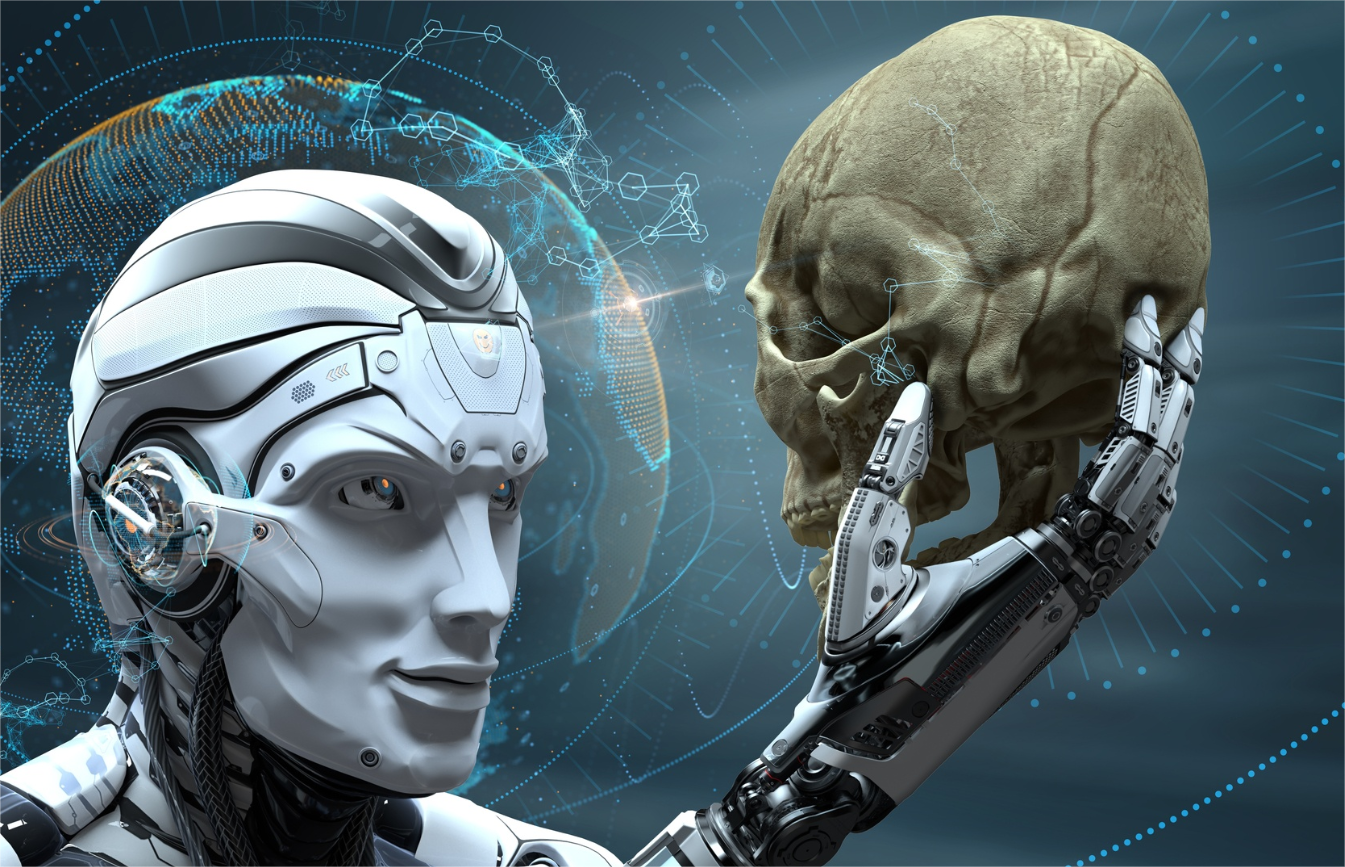
\includegraphics[width=10cm]{imagens/serounaoser.png}\\
  %  \caption{Ser ou não ser}
 %   \label{fig:enter-label}
%\end{figure}
\begin{abstract}


 Este trabalho foi realizado no âmbito da disciplina de \ac{IEI} do curso \ac{leci}.
\vspace{5pt}

O trabalho investiga a \ac{IA}, um ramo da ciência da computação que revolucionou a forma como os seres humanos enfrentam problemas e tarefas complexas. O trabalho, traça a história da \ac{IA} desde as suas raízes na filosofia, passando pelos marcos tecnológicos importantes ao longo do tempo, até às suas utilizações modernas no século XXI. Além disso, aborda como a \ac{IA} funciona e explica em detalhe tecnologias-chave da mesma. Essas tecnologias permitem a capacidade de aprender a partir de dados, reconhecer padrões, interpretar a linguagem humana e processar informação visual, aplicando-se a indústrias tão diversas como saúde, transportes, entretenimento e finanças.
\vspace{5pt}

A \ac{IA} pode apoiar as pessoas em várias áreas: execução de tarefas rotineiras, melhoria de diagnósticos médicos, habilitação de assistentes virtuais e veículos autónomos. No entanto, todas estas melhorias trazem novos desafios, como dilemas éticos, questões de privacidade de dados e vulnerabilidades de segurança. Este trabalho avalia criticamente esses riscos e reforça a necessidade urgente de regulamentações e princípios éticos para assegurar o uso responsável da \ac{IA}.
\vspace{5pt}

Para além das discussões técnicas e éticas, o estudo também explora a dimensão cultural da \ac{IA}, apresentando a sua influência em mídia como videojogos, como \textit{Detroit: Become Human}, e filmes, como \textit{2001: Odisseia no Espaço}. Os testemunhos de especialistas, como Stephen Hawking e Elon Musk, oferecem perspetivas variadas, desde um otimismo cauteloso até alertas sobre os riscos da \ac{IA}. A conclusão aponta para as enormes oportunidades oferecidas pela \ac{IA}, mas destaca que o impacto final dependerá das decisões humanas relacionadas com o seu desenvolvimento, implementação e regulamentação. Assim, o estudo sublinha a necessidade de uma abordagem equilibrada, defendendo a inovação acompanhada de responsabilidade ética como forma de garantir que a \ac{IA} se torne uma ferramenta de progresso e não uma ameaça à sociedade.

\end{abstract}

%%%%%% Agradecimentos %%%%%%
% Segundo glisc deveria aparecer após conclusão...
%\renewcommand{\abstractname}{Agradecimentos}
%\begin{abstract}
%Eventuais agradecimentos.
%Comentar bloco caso não existam agradecimentos a fazer.
%\end{abstract}

\renewcommand{\contentsname}{Índice}
\tableofcontents
%\listoftables     % descomentar se necessário
\listoffigures    % descomentar se necessário


%%%%%%%%%%%%%%%%%%%%%%%%%%%%%%%
\clearpage
\pagenumbering{arabic}

%%%%%%%%%%%%%%%%%%%%%%%%%%%%%%%%
\chapter{Introdução}
\label{chap.introducao}
O desenvolvimento da tecnologia é um dos principais fatores para a evolução e transformação da sociedade ao longo da história humana. Desde pequenas ferramentas, da pré-história, até às grandes criações tecnológicas como o smartphone ou até mesmo o automóvel, que marcaram a nossa forma de viver. 
\vspace{5pt}

A \ac{IA} é um campo da ciência da computação que desenvolve algoritmos e sistemas capazes de realizar tarefas que normalmente requerem inteligência humana, como raciocínio, aprendizagem, planeamento e criatividade. Os sistemas de \ac{IA} são capazes de adaptar o comportamento autonomamente, analisando os procedimentos anteriores. 
\vspace{5pt}

A \ac{IA} foi uma inovação no mundo tecnológico que facilitou a realização de várias tarefas. Embora seja uma grande ajuda e o seu uso tenha várias vantagens, pode se tornar cada vez mais perigosa, pois tem uma potencialidade de evolução muito grande. É essencial utilizar esta ferramenta com cuidado e com consciência, não ficando dependente da mesma. 
\vspace{5pt}

Este documento está dividido em nove capítulos. A introdução ao qual corresponde o  \autoref{chap.introducao}. No \autoref{chap.história} é apresentada a história da \ac{IA} seguida do seu funcionamento, no \autoref{chap.funcionamento}. No \autoref{chap.técnicas}, falamos sobre algumas técnicas usadas para trabalhar com \ac{IA}. As potencialidades da \ac{IA} no \autoref{chap.potência} e os seus perigos no \autoref{chap.perigos}, para exemplificar decidimos incluir um novo capitulo, \autoref{chap.curiosidades}, ao qual damos vários exemplos. Incluímos também um capítulo dedicado a testemunhos/opiniões de pessoas relevantes para o ramo que estamos a desenvolver, no \autoref{chap.testemunhos}. Finalmente, no \autoref{chap.conclusões} são apresentadas as conclusões do trabalho.



%\chapter{Metodologia}
%\label{chap.2}
%Descreve os métodos utilizados para obtenção de resultados.

%Neste esqueleto de relatório aproveitamos este capítulo para exemplificar
%como se usam alguns elementos de {\LaTeX}.

%\section{Exemplos}

%\subsection{Utilização de acrónimos}
%Esta é a primeira invocação do acrónimo \ac{ua}.
%E esta é a segunda \ac{ua}.
%\ac{ML} e \ac{TP}
%Outra referência à \ac{leci}.

%\subsection{Referências bibliográficas}
%Informação relativa à estrutura formal de um relatório pode ser obtida
%na página do \ac{glisc}\cite{glisc}.


\chapter{História}
\label{chap.história}
Enquanto conceito, a \ac{IA} teve origem na filosofia, ou no pensamento humano, não sendo possível definir uma data em concreto. Inicialmente, surgiu com forma abstrata, permitindo espaço para inúmeras análises, frequentemente alicerçadas na (eventual) existência de Deus, no seu poder de criação e na condição humana.

René Descartes, um matemático, filósofo e cientista, apresentou alguns pontos de vista interessantes no seu livro "\textit{Discourse on the Method}"\cite{DoM}, relativamente às capacidades futuras da \ac{IA} e onde se poderiam delinear os seus limites. Este defendia que a capacidade humana para pensar estava intrinsecamente associada à alma, a qual apenas poderia ser criada por Deus. Perante esta ideia, infere-se que uma máquina nunca igualaria o nível do raciocínio humano. 

Apesar de este tipo de noções se terem baseado em grande parte na razão e nas crenças, inúmeras questões, que outrora eram consideradas marcantes e inovadoras, permanecem na atualidade e iram continuar a permanecer no futuro como importantes pontos de vista, principalmente no que diz respeito à aplicabilidade da ética e da moral neste campo, já integrado no quadro científico.
\vspace{10pt}
\begin{figure}[ht]
    \centering
    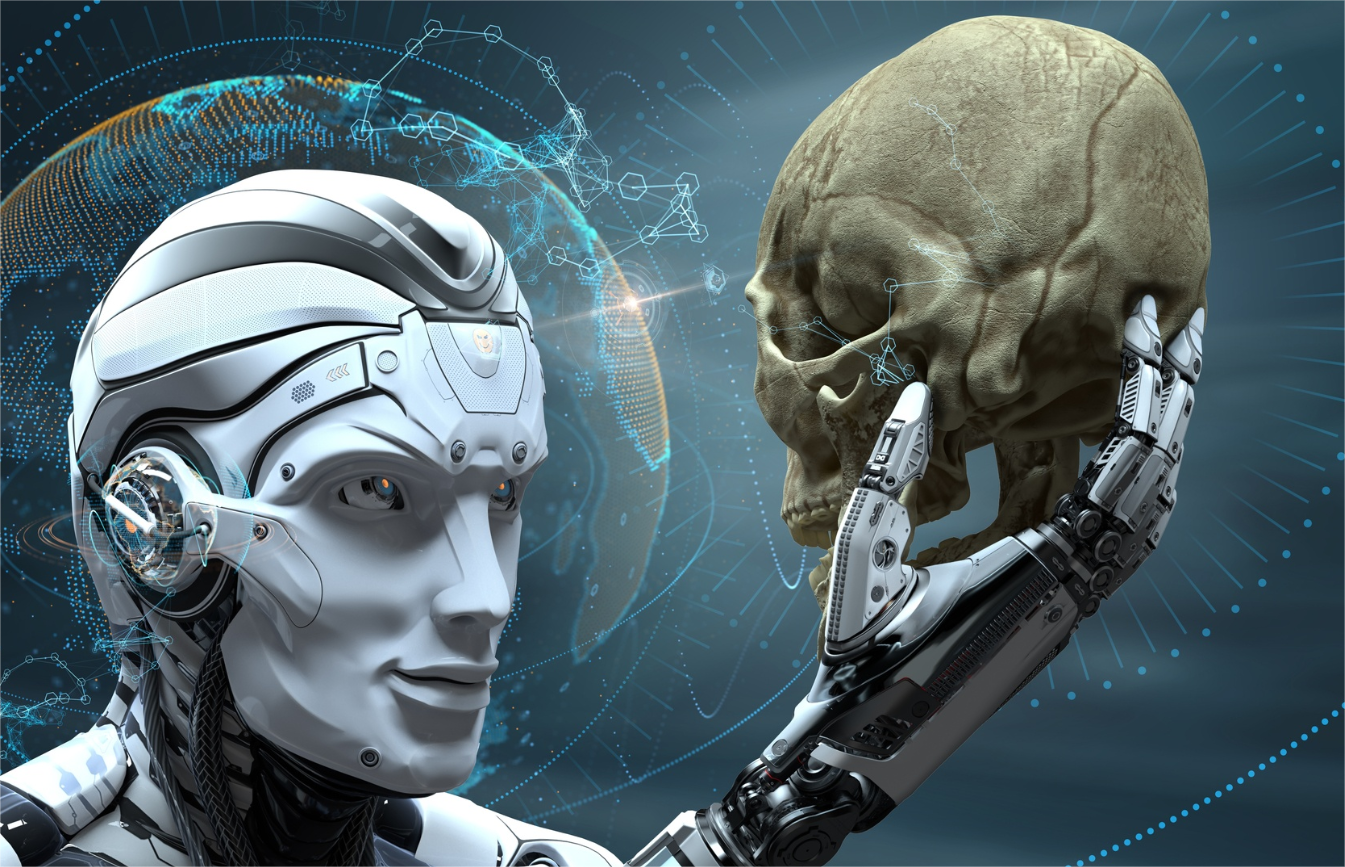
\includegraphics[width=0.7\linewidth]{imagens/serounaoser.png}
    
\end{figure}

\section{Década de 1940}

Em 1943, Walter Pitts \ref{fig:walter} e Warren McCulloch \ref{fig:warren} apresentaram um modelo matemático capaz de representar o funcionamento dos neurónios no cérebro humano. Graças a este modelo revolucionário foi possível a construção de redes neurais artificiais, que são capazes de aprender a partir de informação fornecida, melhorar as suas competências ao longo do tempo.

\begin{figure}[ht]
    \centering
    \subfloat[\label{fig:walter}]{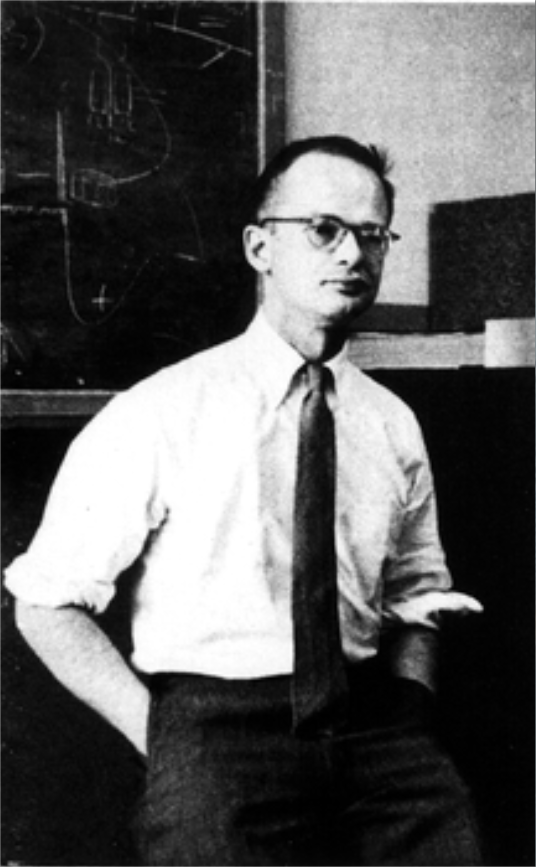
\includegraphics[width=0.311\textwidth]{imagens/WalterPitts.png}}
    \subfloat[\label{fig:warren}]{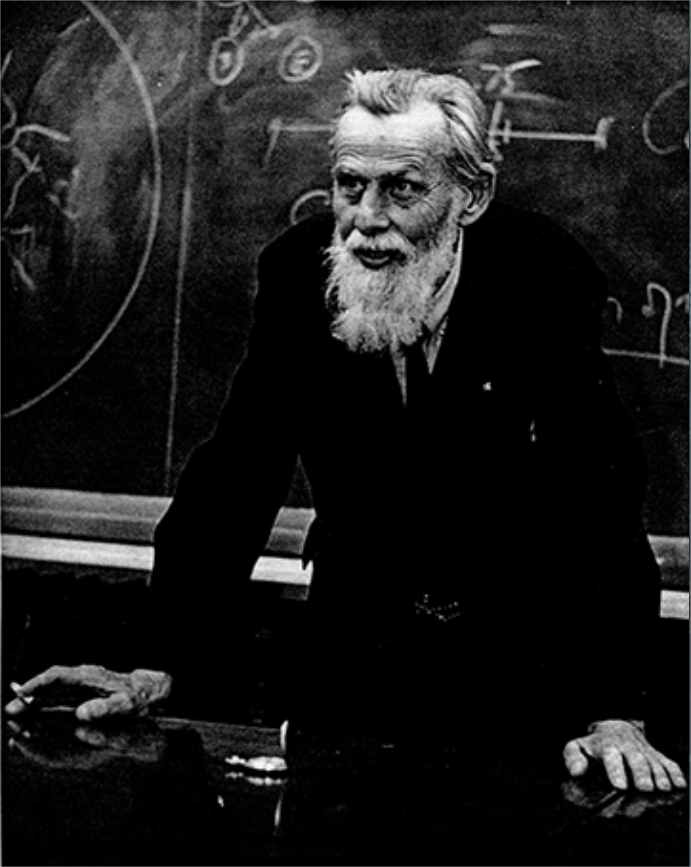
\includegraphics[width=0.4\textwidth]{imagens/WarrenMcCulloch.png}}
    \caption{}
    
\end{figure}

\section{Década de 1950}

\begin{wrapfigure}{r}{0.4\textwidth} 
   \centering
    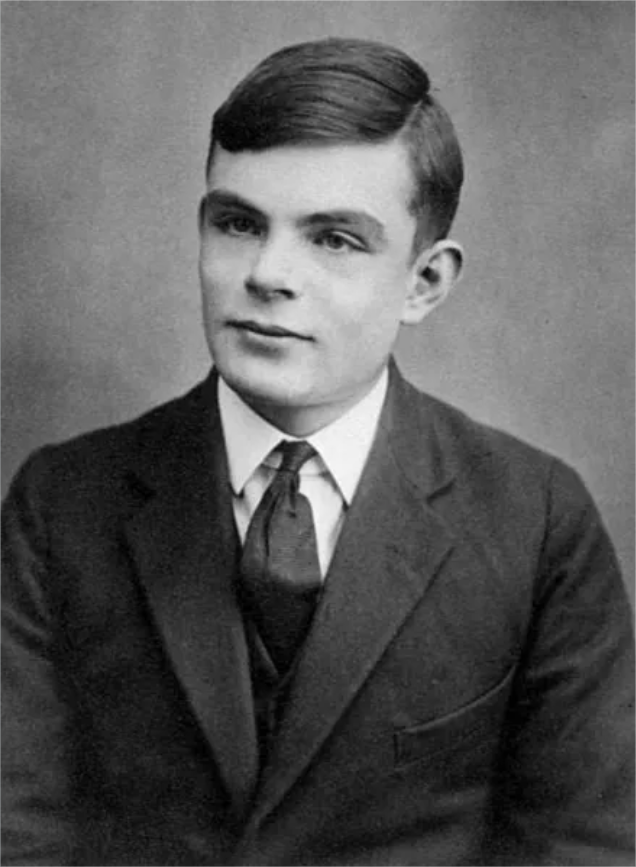
\includegraphics[width=0.3\textwidth]{imagens/Turing.png}
    \footnotesize{\caption{Alan Turing}}
    \label{fig:turing}
\end{wrapfigure}
\vspace{30pt}
Em 1950, Turing propôs o “\textit{Teste de Turing}”, também conhecido como o “Jogo da Imitação”. Este teste propunha que a verdadeira inteligência poderia ser demonstrada se uma máquina conseguisse fazer-se passar por um ser humano, durante uma conversa escrita e tentar enganar um humano.
\\
 Turing, com o seu trabalho, impulsionou a pesquisa sobre \ac{IA}, estabelecendo a questão central de como podemos definir e avaliar a inteligência das máquinas. 
\clearpage
\begin{center}
    \Large\textbf{Teste de Turing}
\end{center}
Em 2014, pela primeira vez, um programa de computador enganou um número considerável de júris no \textit{Teste de Turing}. Ao tentar distinguir uma máquina de um humano, 10 dos 30 júris foram convencidos de que o programa era um humano, mas na realidade tratava-se de uma máquina.

O termo “inteligência artificial” foi usado pela primeira vez em 1956, numa conferência de Dartmouth, para descrever o objetivo de criar máquinas que pudessem demonstrar inteligência semelhante à humana.
\begin{figure}[ht]
    \centering
    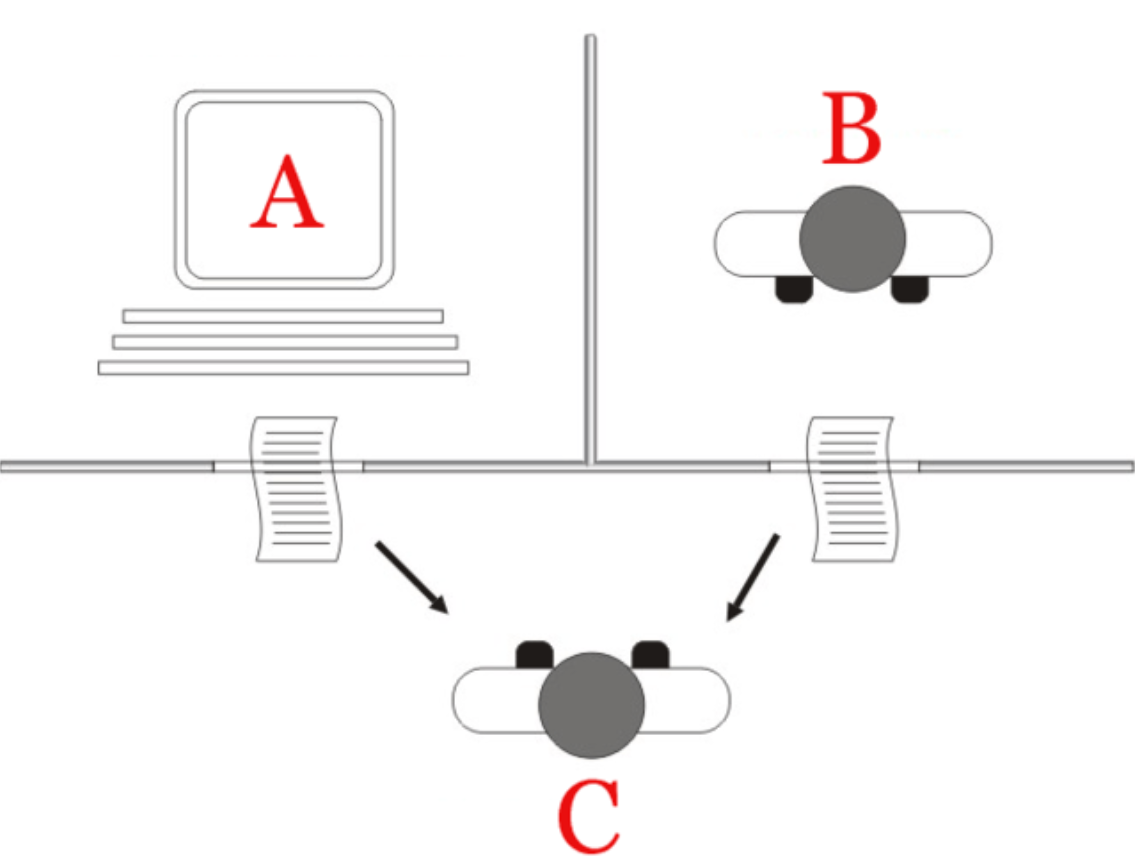
\includegraphics[width=0.4\linewidth]{imagens/testeturing.png}
    \caption{Teste Turing}
    \label{fig:turingtestl}
\end{figure}

\vspace{20pt}

\section{Década de 1960 e 1970}
Durante este período, houve um otimismo inicial sobre o potencial da \ac{IA}, mas também desafios significativos. As limitações computacionais e a falta de dados de treinamento adequados dificultaram o progresso. No entanto, várias técnicas e abordagens, como redes neurais e sistemas especialistas, foram desenvolvidas e aplicadas em diversas áreas.
\begin{figure}[ht]
    \centering
    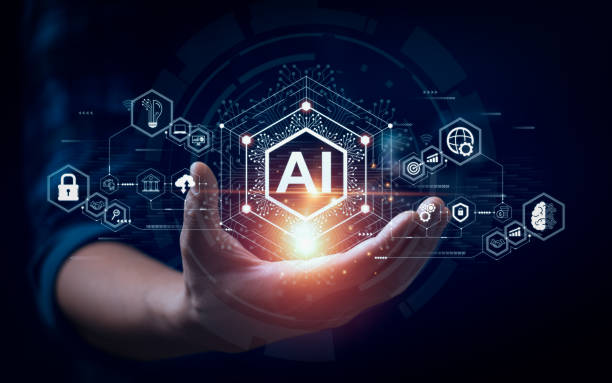
\includegraphics[width=0.6\linewidth]{imagens/ainamao.jpg}
    \caption{AI}
    \label{fig:ainamao}
\end{figure}
\clearpage

\section{Década de 1980 e 1990}

\vspace{10pt}

Nesta época, houve avanços notáveis em áreas como o processamento de linguagem
natural, visão computacional e sistemas especialistas. No entanto, o progresso da \ac{IA} foi irregular, com períodos de entusiasmo seguidos de períodos de desilusão, conhecidos como “invernos da \ac{IA}”,\autoref{fig:inverno}, quando o financiamento e o interesse diminuíram devido a expectativas não atendidas.
\begin{figure}[ht]
    \centering
    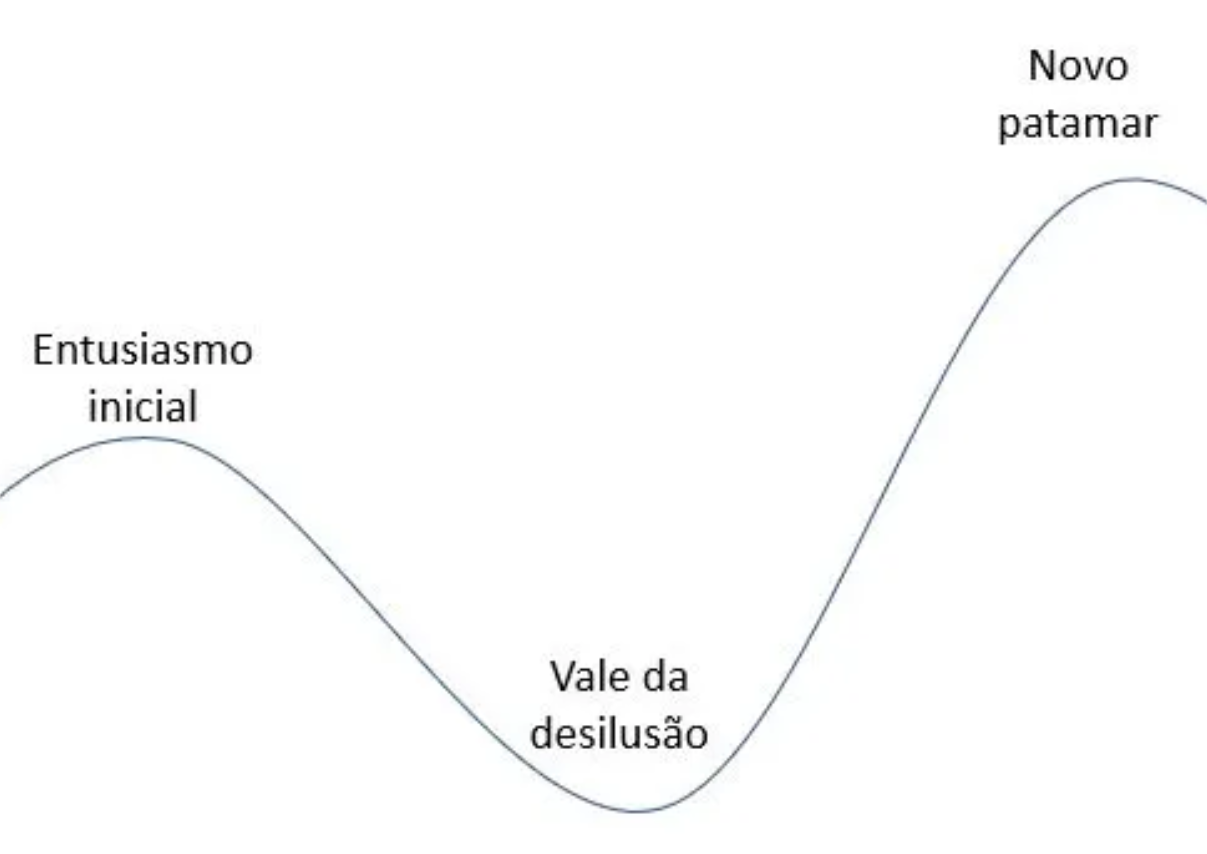
\includegraphics[width=0.5\linewidth]{imagens/aialongthetime.png}
    \caption{}
    \label{fig:inverno}
\end{figure}

\section{Século XXI}
\vspace{10pt}

Atualmente, a \ac{IA} está a ter um crescimento significativo, impulsionado avanços
tecnológicos e a crescente demanda por soluções inteligentes. Um exemplo notável desse avanço é o Chat GPT, uma das aplicações de \ac{IA} mais conhecidas. O Chat GPT, desenvolvido pela OpenAI, utiliza a tecnologia de processamento de linguagem natural para interagir com os utilizadores de maneira conversacional. Essa tecnologia tem sido usada em várias áreas, desde assistentes virtuais e suporte ao cliente até chatbots em plataformas de redes sociais.

\begin{figure}[ht]
    \centering
    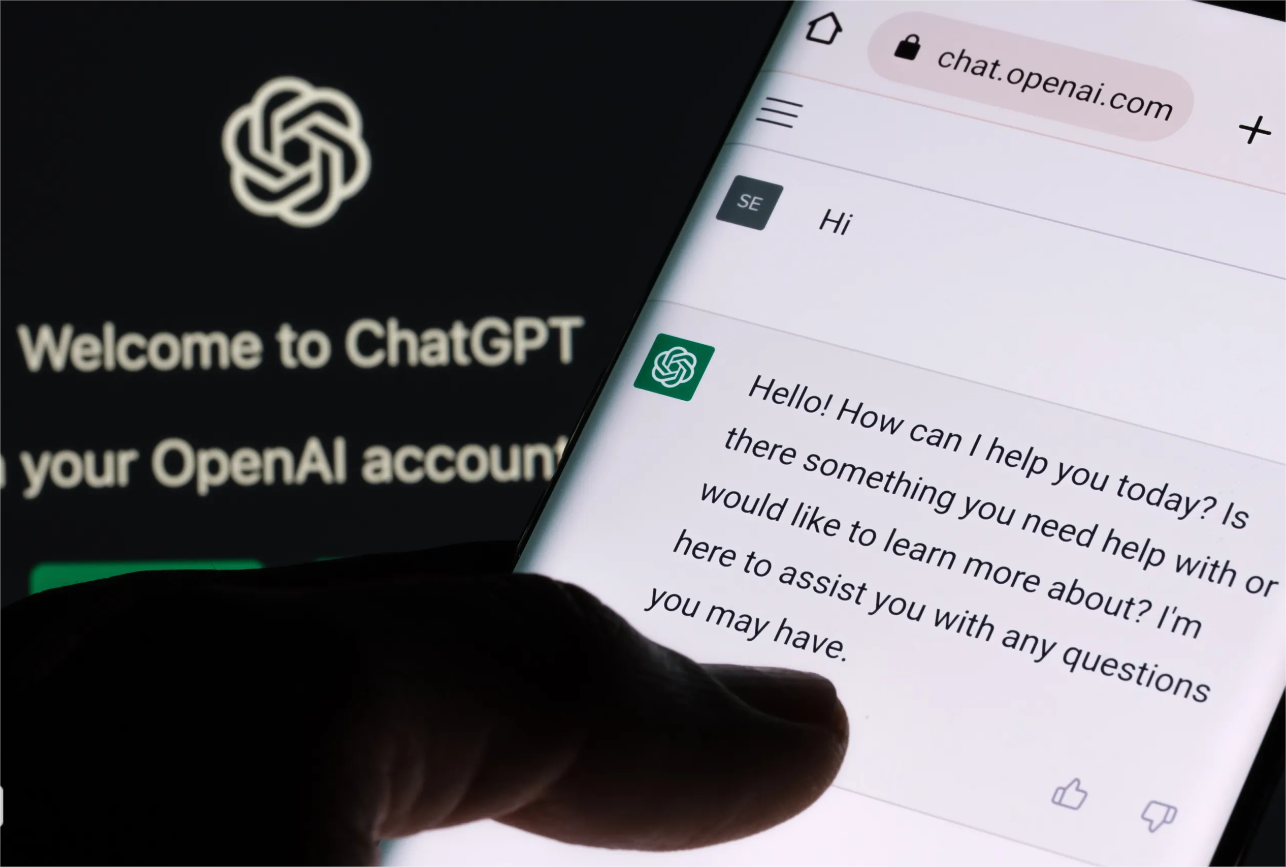
\includegraphics[width=0.5\linewidth]{imagens/chatgpt.png}
    \caption{ChatGPT}
    \label{fig:chatgpt}
\end{figure}


\chapter{Funcionamento da Inteligência Artificial}
\label{chap.funcionamento}
A \ac{IA} funciona através de algoritmos e modelos computacionais que permitem sistemas e programas de computador processem dados, aprendam com esses dados e tomem decisões ou realizem tarefas com base nesse aprendizado.
\begin{description}
    \item[Recolha de dados:] A \ac{IA} depende de dados para aprender e tomar decisões. Esses dados podem ser estruturados (como tabelas de banco de dados) ou não estruturados (como texto, imagens ou áudio).
    \item[Pré-processamento de dados:] Antes que os dados possam ser usados por algoritmos de \ac{IA}, estes precisam de ser pré-processados e preparados. Isso pode incluir limpeza de dados, normalização e transformações para tornar os dados adequados para análise.
    \item[Escolha do algoritmo:] Existem vários algoritmos e técnicas de \ac{IA}, cada um adequado para diferentes tipos de problemas e tipos de dados. A escolha do algoritmo certo depende da natureza do problema a ser resolvido e dos dados disponíveis.

    \clearpage

    
    \item[Treinamento do modelo:] O treinamento de um modelo de \ac{IA} envolve o fornecimento de dados ao algoritmo para que ele possa aprender padrões e fazer previsões ou tomar decisões. Durante o treinamento, o modelo ajusta os seus parâmetros para otimizar o seu desempenho numa tarefa específica.
    \item[Avaliação do modelo:] Após o treinamento, o modelo é avaliado num conjunto separado de dados (conjunto de teste) para verificar se ele é capaz de generalizar para novos dados e se está produzindo resultados precisos.
    \item[Implantação e inferência:] Uma vez treinado e avaliado, o modelo de \ac{IA} pode ser implantado num ambiente de produção, onde pode fazer previsões ou tomar decisões em tempo real com base nos novos dados de entrada.
    \item[Feedback melhoria contínua:] A \ac{IA} pode ser ajustada e melhorada ao longo do tempo com feedback adicional e novos dados de treinamento. Esse processo de melhoria contínua é fundamental para manter a relevância e o desempenho do sistema de \ac{IA} ao longo do tempo.
\end{description}
\begin{figure}[ht]
    \centering
    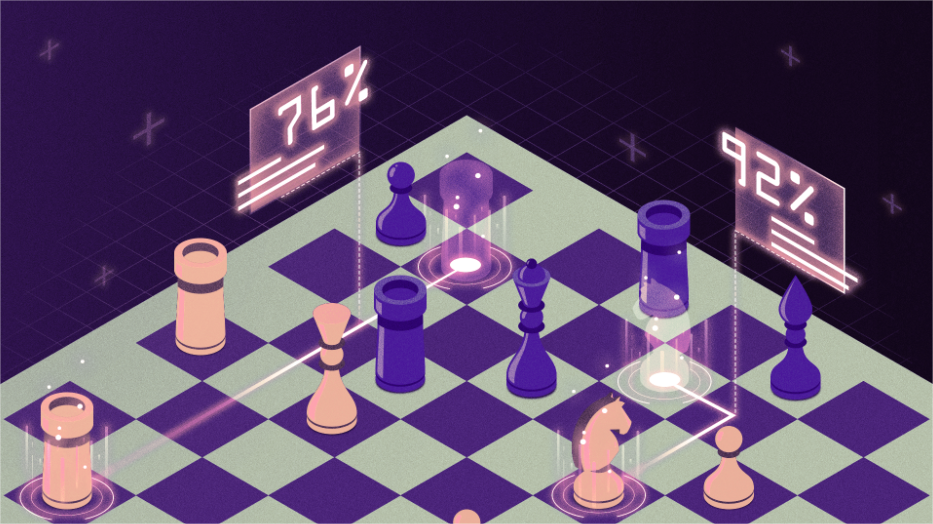
\includegraphics[width=0.8\linewidth]{imagens/xadrez.png}
    \caption{}
    \label{fig:xadreztreinamentoai}
\end{figure}

\chapter{Técnicas usadas para trabalhar com Inteligência Artificial}
\label{chap.técnicas}


\section{Machine Learning}
É uma aplicação de \ac{IA} que fornece aos sistemas de computador a capacidade de aprender e melhorar automaticamente com a experiência, não sendo explicitamente programado. O Machine Learning foca no desenvolvimento de algoritmos que podem analisar dados e fazer previsões.
\vspace{5pt}

Exemplos do uso de Machine Learning:
\begin{itemize}
    \item Sugestão de filmes, na Netflix, que o utilizador pode gostar;
    \item Auxílio no diagnóstico de doenças, interpretação de imagens médicas e aceleração no desenvolvimento de medicamentos;
\end{itemize}
\begin{figure}[ht]
    \centering
    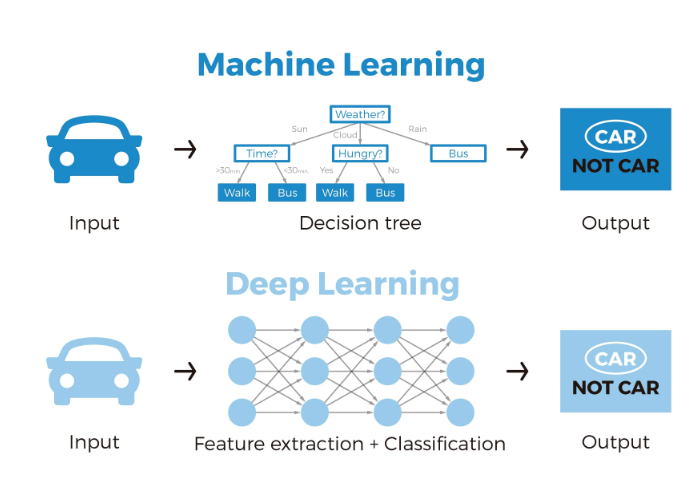
\includegraphics[width=0.4\linewidth]{imagens/machinelearning.png}
    \caption{}
    \label{fig:machine}
\end{figure}
\clearpage

\section{Deep Learning}
É um segmento específico do Machine Learning. O Deep Learning emprega redes neurais artificiais que aprendem através do constante processamento de dados (reforço positivo e reforço negativo). As redes neurais artificiais imitam as redes neurais biológicas do cérebro humano. O Deep Learning é a técnica que leva ao reconhecimento de fala.

\section{Computação cognitiva}
Tem como objetivo imitar e melhorar a interação entre humanos e máquinas. A computação cognitiva procura recriar o processo de pensamento humano num modelo de computador, especificamente, por meio da compreensão da linguagem e do significado das imagens.
A junção da computação cognitiva e da inteligência artificial confere às máquinas comportamentos semelhantes aos humanos e habilidades de processamento de informações.

\section{Natural Language Processing}
\ac{NLP}, permite que os computadores interpretem, reconheçam e produzam a linguagem e a fala humanas.
O objetivo desta técnica é permitir a interação contínua com as máquinas, ensinando os sistemas a compreender a linguagem humana no contexto e produzir respostas lógicas. Uns bons exemplos são tradutores de idiomas em tempo real.

\section{Visão Computacional}
É uma técnica que implementa o Deep Learning e a identificação de padrões para interpretar o conteúdo de uma imagem. A ação é feita entre os mais diversos tipos, incluindo os gráficos, tabelas e imagens em documentos PDF, bem como outros textos e vídeos.


\chapter{Potencialidades da Inteligência Artificial}
\label{chap.potência}
\vspace{25pt}
\Large\textbf{Algumas potencialidades da \ac{IA} são:}\normalsize
\begin{description}
    \item[Automatização de tarefas repetitivas:]  Pode ser usada para automatizar tarefas rotineiras e repetitivas, permitindo recursos humanos para atividades mais criativas e estratégicas;
    \item[Análise de dados complexos:] A análise grandes volumes de dados de forma rápida e eficiente, identificando padrões, tendências e insights que podem ser utilizados para tomar decisões informadas;
    \item[Assistência virtual:] Assistentes virtuais baseados em \ac{IA}, como chatbots e assistentes de voz, podem fornecer suporte e assistência aos usuários numa ampla variedade de tarefas, desde responder a perguntas simples até auxiliar em transações complexas;

    \begin{figure}
        \centering
        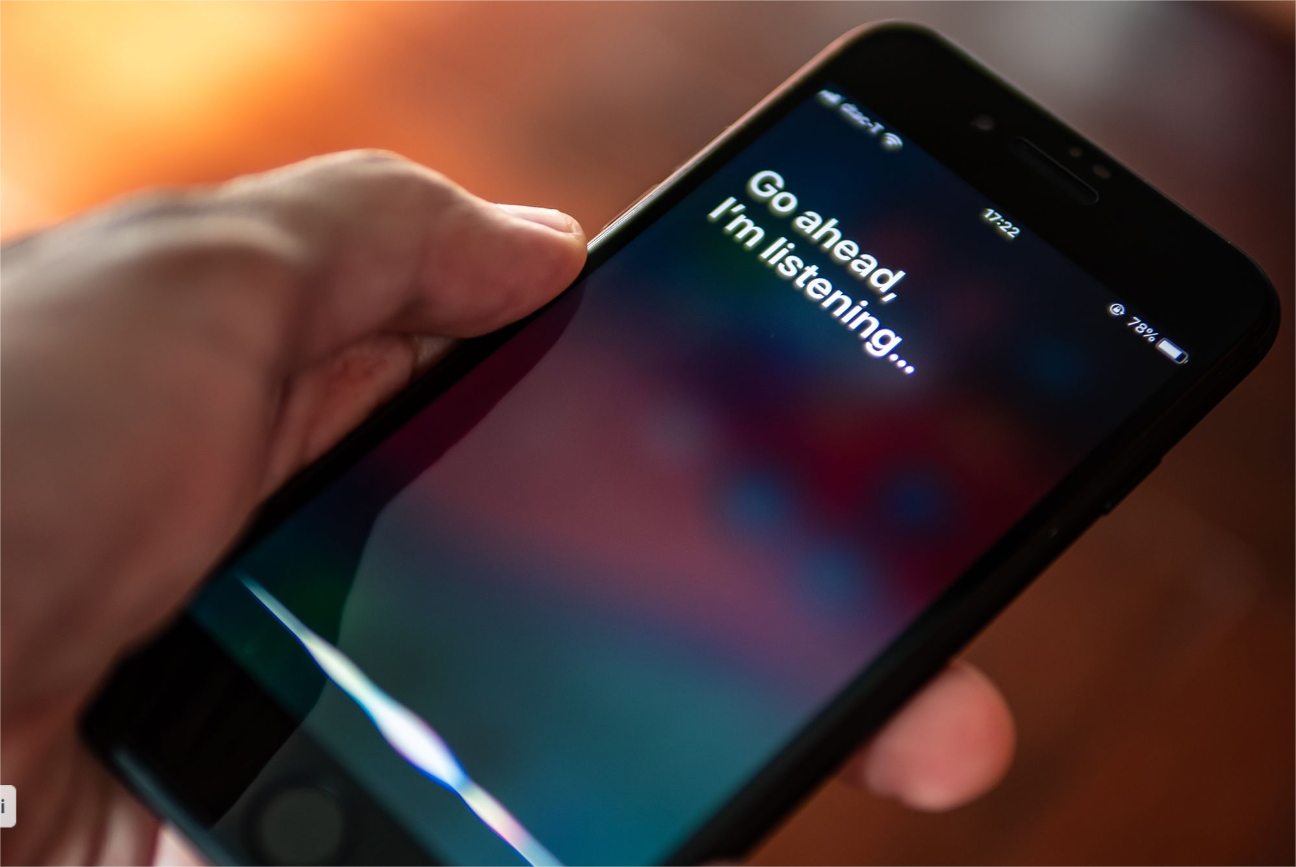
\includegraphics[width=0.5\linewidth]{imagens/siri.png}
        \caption{}
        \label{fig:siri}
    \end{figure}
        
    \clearpage
    
    \item[Reconhecimento de padrões e imagens:] A \ac{IA} pode ser usada para reconhecer padrões em dados de imagens e vídeo, o que é útil em diversas áreas, como diagnóstico médico, vigilância de segurança, reconhecimento facial, entre outros;
    \item[Tradução de idiomas:] A IA pode ser usada para traduzir texto entre diferentes idiomas de forma rápida e precisa, facilitando a comunicação global;
    \item[Aprendizado de máquina:] Algoritmos de aprendizado de máquina permitem que sistemas de \ac{IA} aprendam com os dados e melhorem o seu desempenho ao longo do tempo, sem a necessidade de programação explícita;
    \item[Condução autónoma:] A \ac{IA} é essencial para o desenvolvimento de veículos autónomos, permitindo que estes percebam o ambiente ao seu redor e tomem decisões em tempo real para navegar com segurança
\end{description}.
\begin{figure}[ht]
        \centering
        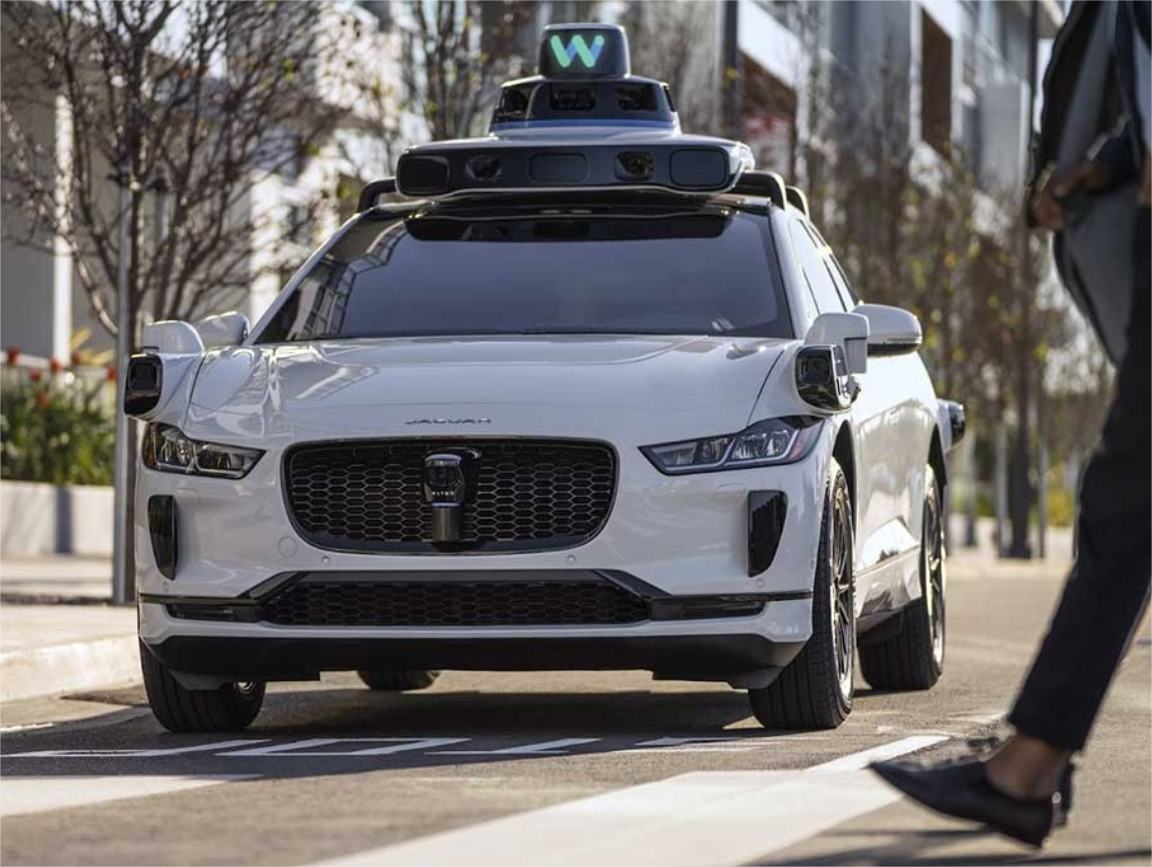
\includegraphics[width=0.6\linewidth]{imagens/taxiautonomo.png}
        \caption{}
        \label{fig:Carro}
    \end{figure}
\vspace{5pt}


\chapter{Perigos da Inteligência Artificial}
\label{chap.perigos}

A \ac{IA} tem despertado grandes expectativas e gerado discussões acaloradas em vários setores da sociedade. A sua capacidade de processar grandes volumes de dados, aprender com padrões complexos e tomar decisões autónomas promete transformar radicalmente a forma como vivemos e trabalhamos, demonstrando claramente as vantagens da \ac{IA}. Desde diagnósticos médicos mais precisos a carros autónomos que prometem revolucionar o transporte, os benefícios da \ac{IA} são vastos e variados.
No entanto, à medida que a \ac{IA} se torna uma presença cada vez mais omnipresente nas nossas vidas, somos também confrontados com uma série de desafios e preocupações que precisam de ser abordados com urgência, demonstrando claramente que existem também os malefícios da \ac{IA}. 
\vspace{10pt}

Alguns perigos da \ac{IA} são:
\begin{description}
    \item[Segurança:]
    
    Um dos principais riscos associados à \ac{IA} é a segurança do sistema. Com a crescente dependência de algoritmos e sistemas autónomos, existe uma preocupação significativa com a possibilidade de ataques cibernéticos dirigidos a estes sistemas.
    Seja manipulando algoritmos para resultados maliciosos ou explorando vulnerabilidades em sistemas autónomos, os ciberataques representam uma ameaça real à segurança da \ac{IA}, provando ser um dos maiores perigos da \ac{IA}.
    \item[Privacidade de dados:]
    
    Com a capacidade da \ac{IA} de recolher, analisar e interpretar grandes volumes de dados, surgem preocupações significativas com a privacidade. O uso indevido ou violação de dados pessoais pode ter consequências graves para os indivíduos, incluindo o risco de discriminação algorítmica e violações de privacidade.
    
    \clearpage

    
    \item[Ética:]
    
    A \ac{IA} levanta questões éticas complexas, especialmente quando se trata de tomar decisões autónomas que afetam a vida das pessoas. De algoritmos de recrutamento a sistemas de justiça criminal, é crucial garantir que a \ac{IA} seja usada de forma ética e justa.
    Para abordar questões éticas na \ac{IA}, é importante desenvolver diretrizes e regulamentos claros que orientem o desenvolvimento responsável e o uso da tecnologia. Além disso, a transparência algorítmica — ou seja, tornar os algoritmos compreensíveis, para isso é essencial para garantir a responsabilização e a confiança pública na \ac{IA}.
    \item[Controlo:]
    
    Com a rápida evolução da \ac{IA}, existe a necessidade de uma governação eficaz para garantir que esta tecnologia seja utilizada de forma responsável e benéfica para a sociedade como um todo. Isso inclui questões relacionadas à regulamentação, supervisão e responsabilização dos sistemas de \ac{IA}.
    Para promover uma governação eficaz da \ac{IA}, é necessário um diálogo colaborativo entre governos, empresas, académicos e sociedade civil. Isso pode incluir a criação de órgãos reguladores especializados em \ac{IA} e a elaboração de normas éticas e legais que orientem o desenvolvimento e uso da tecnologia.
    \item[Impacto social e económico:]
    
    A \ac{IA} tem potencial para causar um impacto significativo na sociedade e na economia, considerando questões como o emprego e o aumento da automação. Estas mudanças podem gerar tensões sociais e económicas, exigindo uma resposta cuidadosa por parte dos governos e organizações.
\end{description}

\begin{figure}[ht]
    \centering
    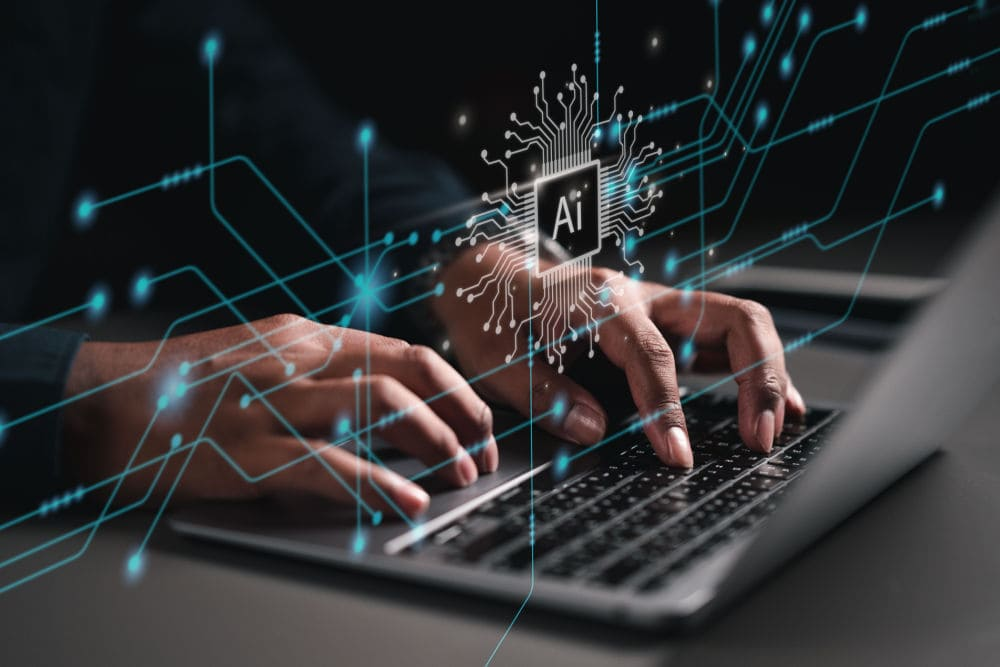
\includegraphics[width=0.5\linewidth]{imagens/plataformas-criar-inteligencia-artificial.jpg}
    \caption{}
    \label{fig:AIi}
\end{figure}

\chapter{Curiosidades}
\label{chap.curiosidades}

\begin{center}
    \Huge{\textbf{Xadrez}}
\end{center}
\vspace{20pt}

Garry Kasparov é um Grande Mestre do xadrez, ex-campeão do mundo no mundo do xadrez. Por muitos é considerado um dos maiores, se não, o melhor jogador de xadrez de todos os tempos. É admirado pelos fãs de xadrez pelas suas conquistas. Foi em 1985, com 22 anos, o jogador mais novo a conquistar o título de campeão do mundo e lutou e manteve o título até 1993. 
\vspace{5pt}
\begin{wrapfigure}{r}{0.5\textwidth} 
   \centering
    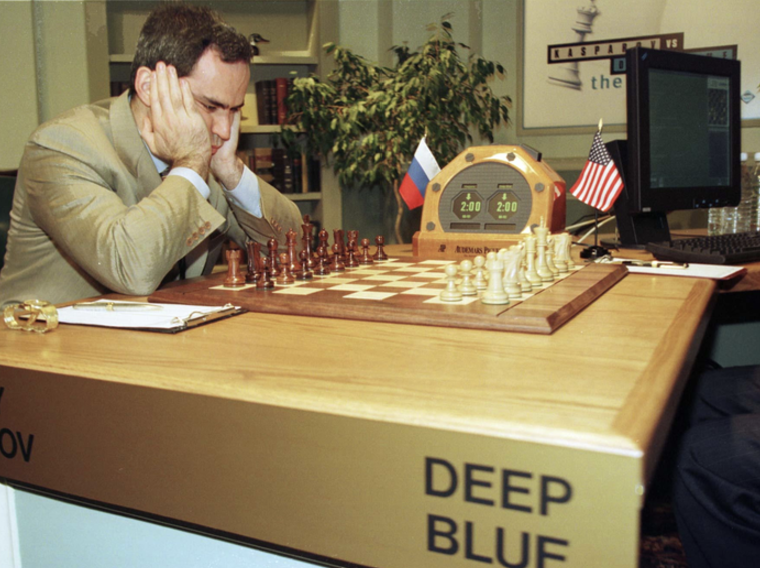
\includegraphics[width=0.4\textwidth]{imagens/chessmatch.png}
    \tiny{\caption{}}
    \label{fig:chess}
\end{wrapfigure}

No ano de 1996, Kasparov realizou 6 jogos contra o computador comandado por IA, ao qual o ex-campeão do mundo conseguiu acabar as 6 partidas com resultado favorável, \(4-2\).

Garry venceu o primeiro confronto contra a máquina. Mas logo no ano a seguir realizou-se em Nova Iorque a desforra, à qual o mesmo supercomputador, Deep Blue, derrotou o Grande Mestre, por \(3.5-2.5\).
 

Foi graças a essa derrota que foi criado um documentário, "\textit{Game Over Kasparov and the Machine}" que relata essa mesma história. 
\vspace{2pt}


Os jogos foram cuidadosamente analisados, e após a vitória, Deep Blue, tornou-se muito famoso. A sua vitória teve um impacto significativo. Pois, foi necessário alguém com um grande impacto em questões de 
intelectualidade, ir a "baixo", neste caso perder um jogo que maioritariamente depende do intelecto do jogador, para que as pessoas percebessem que aquilo já seria um sinal que a inteligência artificial estaria a alcançar a inteligência dos humanos. 
\clearpage
\vspace{100pt}
\begin{center}
    \Huge{\textbf{Pokémon Go}}   
\end{center}

\vspace{20pt}

\begin{wrapfigure}{r}{0.4\textwidth} 
    \centering
    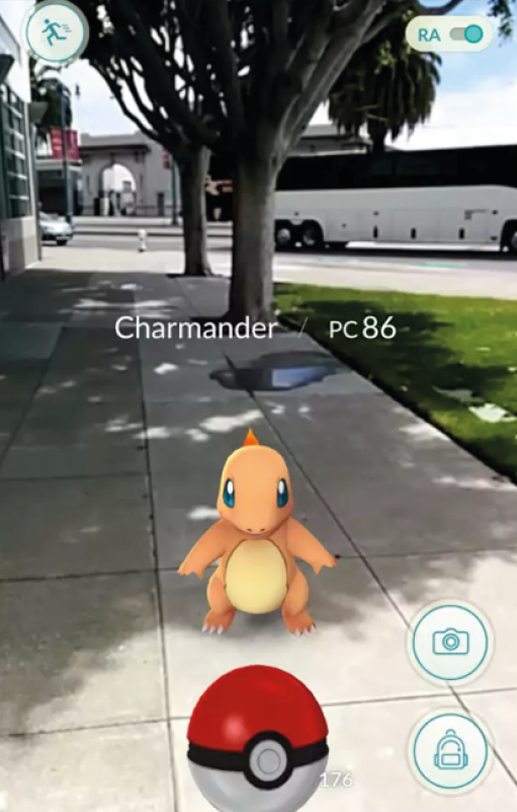
\includegraphics[width=0.3\textwidth]{imagens/pokemongo.png}
    \footnotesize{\caption{Exemplo da RA}}
    \label{poke}
\end{wrapfigure}

Pokemon Go, é um videojogo para dispositivos móveis, tendo sido disponibilizado pela primeira vez em 2016, e desde a sua data de lançamento obteve mais de 600 milhões de downloads.
O jogo consiste em capturar pokémons. Para isso é necessário que o jogador se movimente, a movimentação do personagem no jogo é feita com base na localização real do jogador. 
 Ou seja, isto obriga ao utilizador/jogador sair de casa para progredir no jogo. 
 
\vspace{5pt}

Numa determinada área na vida real, poderão existir mais coisas de interesse no jogo.
Contudo, os pontos de interesse na vida real, como museus, monumentos e lojas, estão associados a recursos no jogo, ou seja, se o jogador se encontrar ao lado de um museu e tirar uma foto ao museu o jogador ganha recursos virtuais, recursos estes que necessita para evoluir.

\vspace{5pt}

Ou mesmo não estando perto de pontos de interesse, o jogo possui um recurso que faz com que através de \ac{RA} o jogador possa observar os seus pokémons no mesmo meio ambiente.

\vspace{5pt}

A empresa criadora do jogo, Niantic, foi acusada de, através de todas estas funcionalidades, poder estar a usa-las para treinar \ac{IA}. Foi afirmado que no mundo todo 10 milhões de localizações já foram analisadas e são feitas cerca de 1 milhão de novas análises através destes recursos.
Como resposta a essa acusação, a Niantic afirmou que “\textit{As funcionalidades que apresentamos no nosso jogo para fazer scan são opcionais…}”. 

Ao cativar os jogadores com benefícios, se fizerem uso destas funcionalidades, torna algo que antes era opcional em algo obrigatório.

\clearpage

\begin{center}
    \Huge{\textbf{Detroid: Become Human}}   
\end{center}
\vspace{50pt}

O videojogo conta a história de 3 robôs criados pela empresa fictícia CyberLife, e ao desenrolar da história, o jogo depende das escolhas que o jogador escolhe que os robôs tomem.
No desenrolar do jogo os robôs, que eram inicialmente controlados pelo seu respetivo humano, após algo inesperado acontecer, estes começam a pensar por eles próprios, aproximando os seus comportamentos cada vez mais aos comportamentos de um ser humano, desenvolvendo uma aproximação dos sentimentos dos humanos com os seus.  

\vspace{40pt}
\begin{figure}[ht]
    \centering
    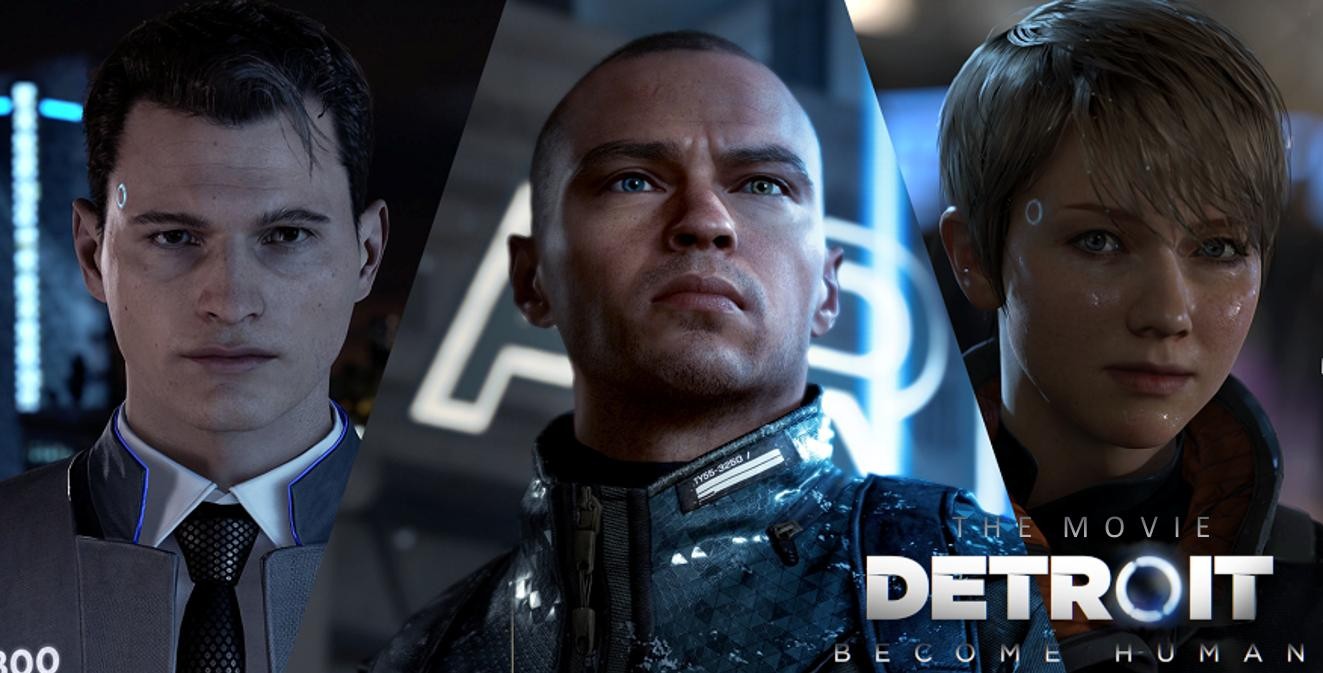
\includegraphics[width=\linewidth]{imagens/Detroit.jpg}
    \caption{}
    \label{fig:detroit}
\end{figure}




\clearpage


\begin{center}
    \Huge{\textbf{Hal 9000}}    
\end{center}

\vspace{20pt}

Lançado em 1968, “\textit{2001: Odisseia no Espaço}” realizado por Stanley Kubrick é um dos filmes mais marcantes da história do cinema. 
Uma experiência que começa na pré-história da Humanidade e passa para uma nave que ruma ao infinito, num drama envolvente da luta do homem contra a máquina.
\vspace{5pt}

No filme, Hal 9000, é a \ac{IA} que controla todos os aspetos da nave espacial Discovery One, que se dirige ao planeta Júpiter, e da vida dos astronautas que viajam a bordo. Embora HAL esteja programado para ajudar e levar os astronautas até o seu destino, a \ac{IA} começa a tomar decisões por conta própria, originando resultados catastróficos. A sua omnipresença e relação com a tripulação destacam a complexa dualidade entre o potencial da tecnologia e os riscos que esta apresenta.
\vspace{5pt}

"I'm sorry Dave, I'm afraid I can't do that".

Estas perturbadoras palavras do computador HAL 9000 definem a ansiedade atualmente predominante sobre o possível domínio da \ac{IA} sobre a humanidade.
\vspace{5pt}

O clássico do realizador Stanley Kubrick explora os avanços da tecnologia, apresentando talvez o cenário mais impressionante do conflito entre a máquina e o ser humano da história do cinema. Mesmo tendo sido lançado em 1968, “\textit{2001: Odisseia no Espaço}” aborda temas muito à frente do seu tempo, e demonstra de forma brilhante um dos maiores problemas com o avanço das tecnologias.
\vspace{40pt}

\begin{figure}[ht]
    \centering
    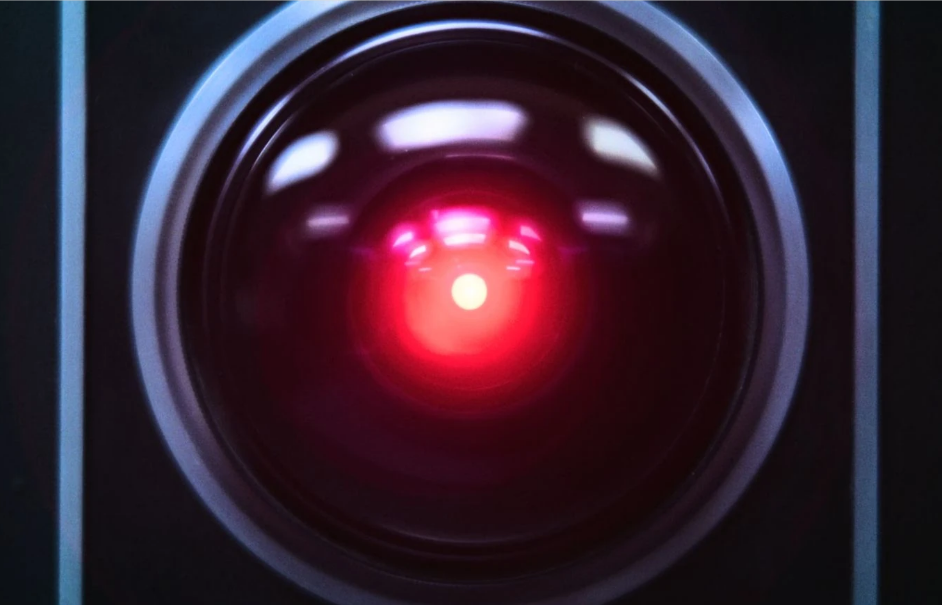
\includegraphics[width=0.8\linewidth]{imagens/hal 9000.png}
    \caption{}
    \label{fig:hal9000}
\end{figure}
\chapter{Testemunhos}
\label{chap.testemunhos}

\begin{center}
    \LARGE{\textbf{Mark Zuckerberg vs Elon Musk}}    
\end{center}

\vspace{15pt}
Com o avançar da tecnologia, os nossos comportamentos enquanto seres humanos, alteraram-se completamente. É raro o dia em que nós não pegamos no telemóvel para abrir as nossas redes sociais, e sem dar mos conta já passamos demasiado tempo agarrados ao ecrã. 

Os algoritmos são os responsáveis por contribuir para esse vício, condicionam o conteúdo que nos é disponibilizado, ou seja, não tem como objetivo disponibilizar a melhor informação mas sim apresenta-nos algo que nos cativa involuntariamente a ficar agarrados ao ecrã.

É com este avanço alarmante que surgem várias questões éticas. 

\vspace{15pt}
A \ac{IA}, é uma ferramenta para nos \textbf{ajudar} ou 
um recurso para nos \textbf{destruir}?  
\vspace{5pt}



\begin{wrapfigure}{r}{0.3
\textwidth} 
    \centering
    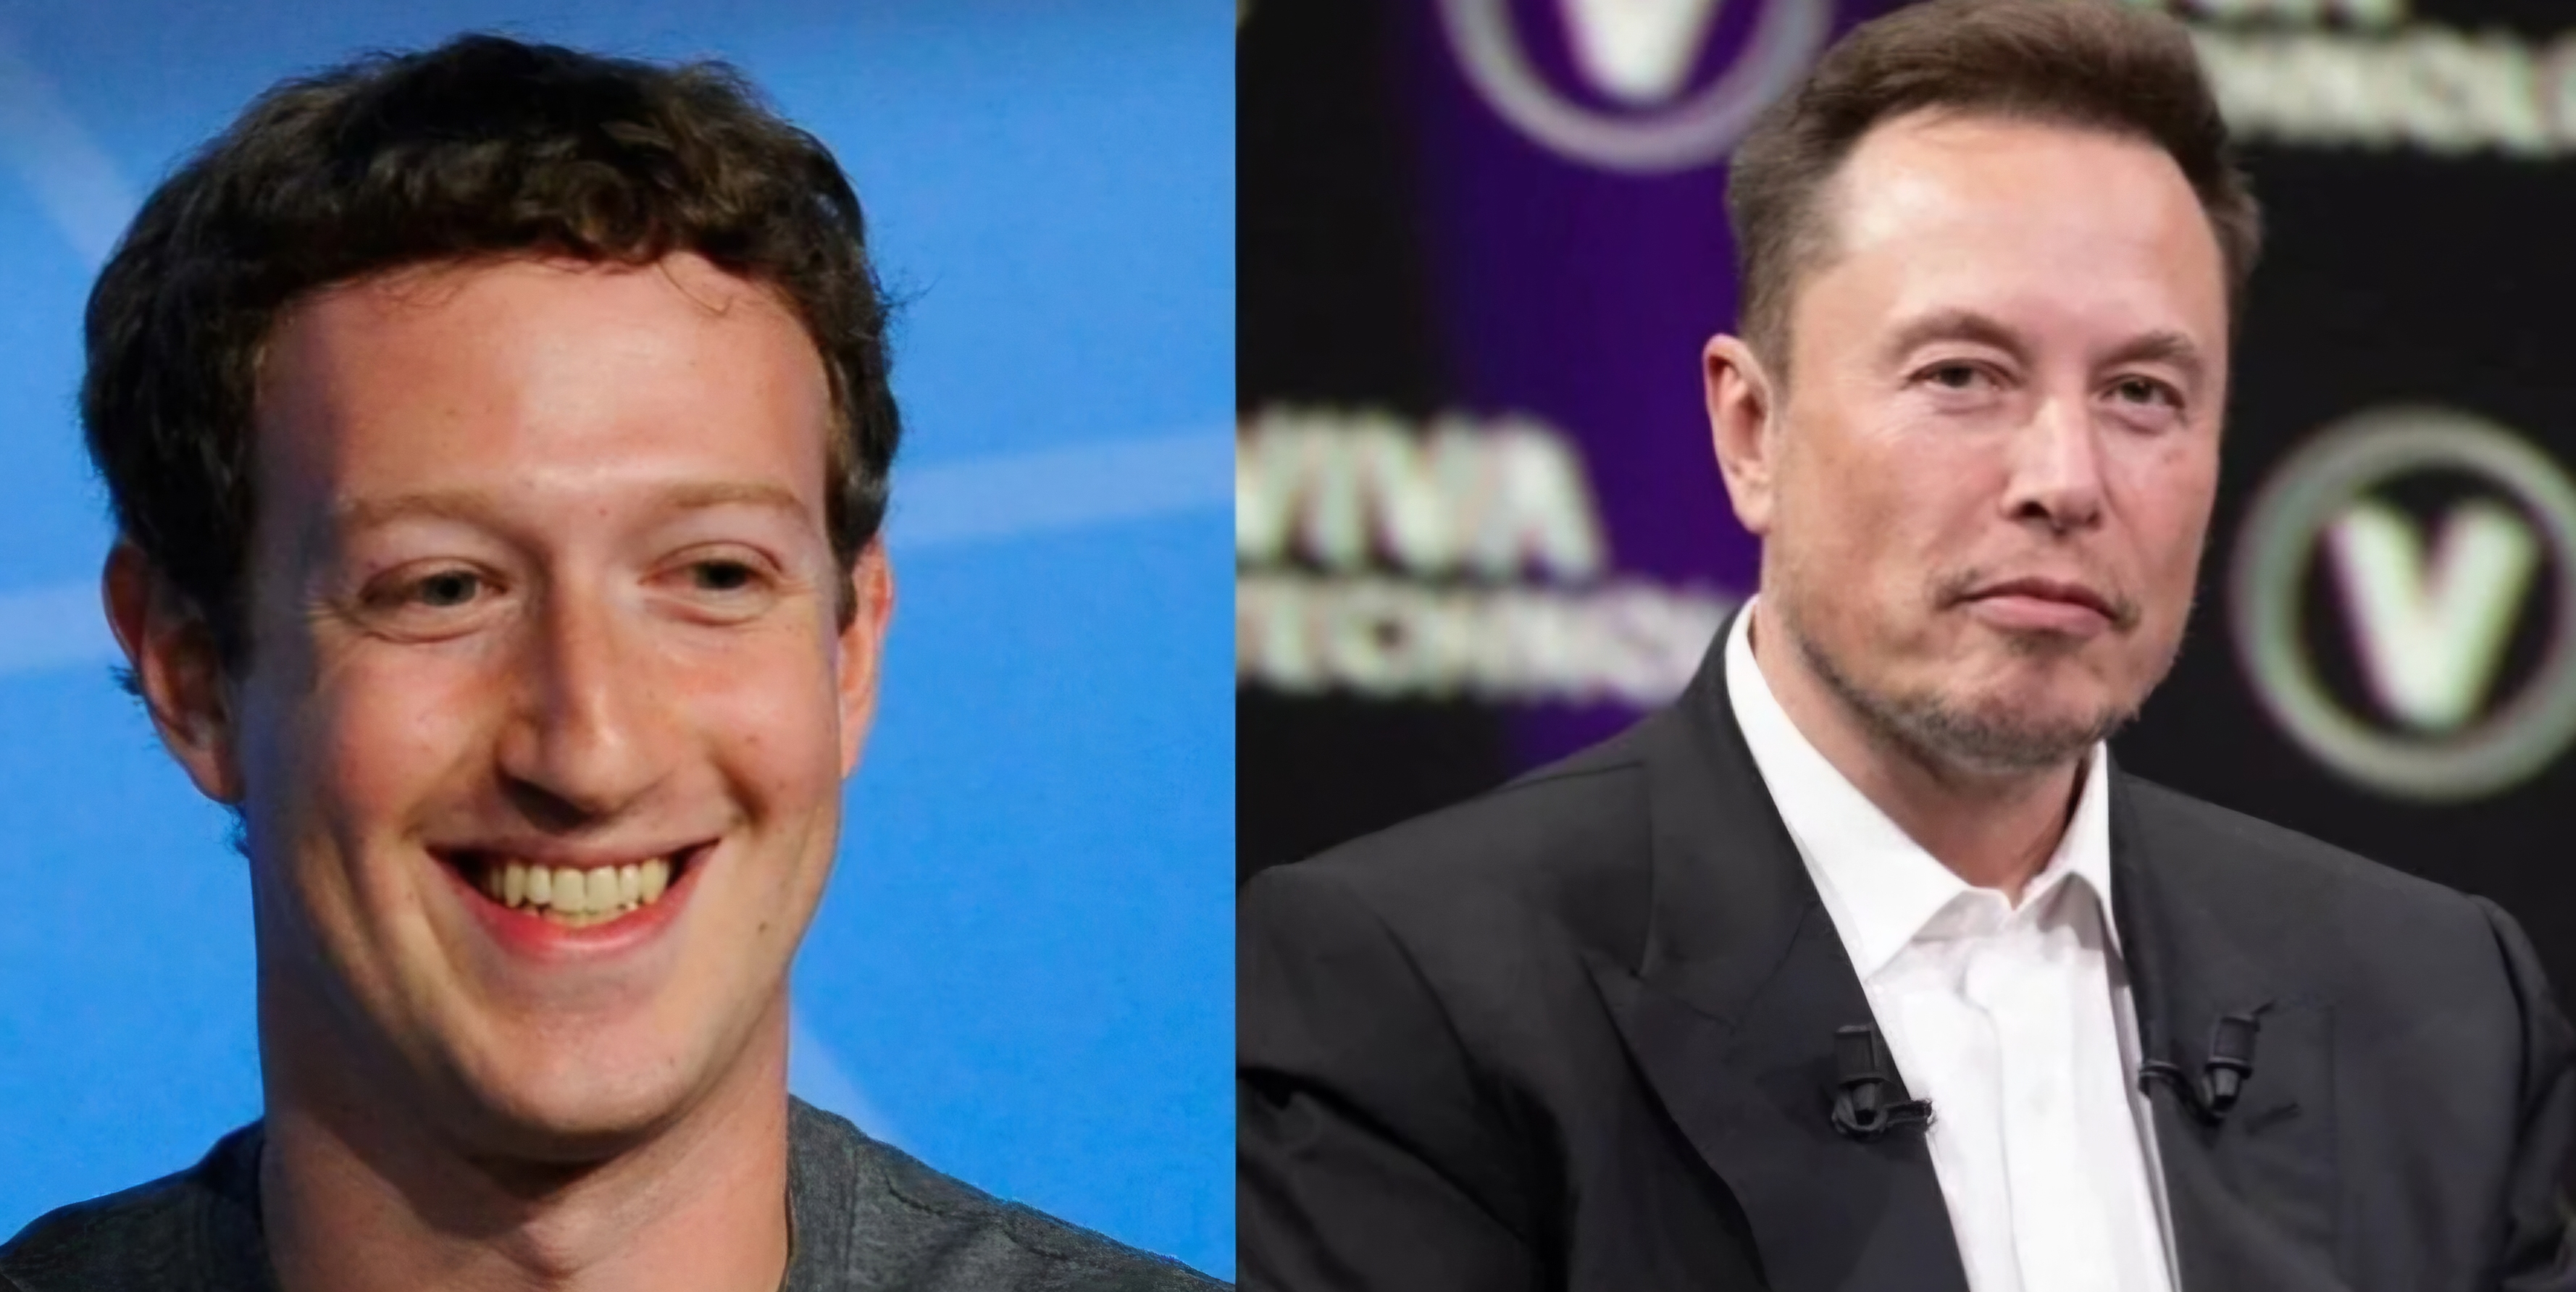
\includegraphics[width=0.3\textwidth]{imagens/marcvsmusk.jpg}
    \footnotesize{\caption{}}
    \label{muskzuc}
\end{wrapfigure}



Neste debate dois dos grandes nomes da área da tecnologia, Mark Zuckerberg e Elon Musk. 

De um lado Mark Zuckerberg criador da rede social Facebook e atual dono das redes Instagram e Whatsapp. Defende a ideia:\\
"\textit{Não vale a pena alarmismos, a \ac{IA} apenas servirá como uma ferramenta para facilitar a realização das nossas tarefas}".

\vspace{10pt}

Por outro lado, Elon Musk, dono da antiga rede social Twitter, fundador da Tesla e da SpaceX, considera que a \ac{IA} será, se já não é, uma ameaça. Ele afirma: \\“\textit{O que nos difere dos outros seres é sermos os únicos a possuir inteligência, aquilo que está acontecer é que estamos a criar algo que será mais inteligente que o ser humano mais inteligente do mundo}”.

\vspace{100pt}

\begin{center}
    \LARGE{\textbf{Stephen Hawking vs Rollo Carpenter}}    
\end{center}

\vspace{15pt}

Stephen Hawking, um dos maiores cientistas do mundo, afirmou numa entrevista, que os esforços para criar máquinas pensantes são uma ameaça à existência humana. Nessa entrevista, constatou que "\textit{O desenvolvimento da \ac{IA} poderia significar o fim da raça humana}". Hawking fez a advertência ao responder a uma pergunta sobre os avanços da tecnologia que ele próprio usa para se comunicar, a qual utiliza uma forma básica de \ac{IA}.

\begin{wrapfigure}{r}{0.3\textwidth} 
    \centering
    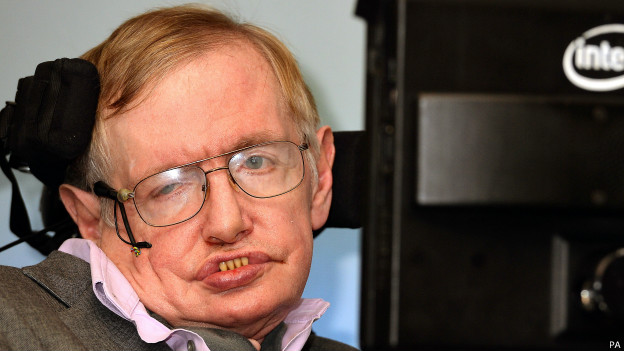
\includegraphics[width=0.3\textwidth]{imagens/stephenhaw.jpg}
    \footnotesize{\caption{}}
    \label{fig:hawking}
\end{wrapfigure}
O físico britânico, que sofre de esclerose lateral amiotrófica, uma doença degenerativa, usa um novo sistema desenvolvido pela empresa Intel para se comunicar. Especialistas da empresa britânica Swiftkey também participaram na criação do sistema. A sua tecnologia, já instalada como uma aplicação para teclados de smartphones, "aprende"\ a forma como Hawking pensa e sugere as próximas palavras que ele poderá querer usar.
\vspace{5pt}

Hawking diz que as formas primitivas de \ac{IA} desenvolvidas até agora têm se mostrado muito úteis, mas teme eventuais consequências ao se criar máquinas que sejam equivalentes ou superiores aos humanos.
"\textit{(Estas máquinas) avançariam sozinhas e redesenhar-se-iam a um ritmo cada vez maior", afirmou. "Os humanos, limitados pela evolução biológica lenta, não conseguiriam competir e seriam superados.}"

\begin{wrapfigure}{l}{0.3\textwidth} 
    \centering
    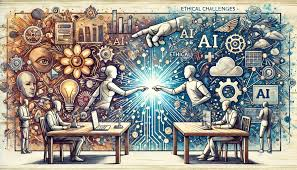
\includegraphics[width=0.3\textwidth]{imagens/conhecimentoeAI.jpg}
    \footnotesize{\caption{}}
    \label{fig:conhecimentoAI}
\end{wrapfigure}


Contudo, nem todos os cientistas, partilham da mesma visão negativa de Hawking sobre a \ac{IA}.
"\textit{Acredito que continuaremos no comando da tecnologia por um período razoável de tempo, e o potencial dela de resolver muitos dos problemas mundiais será concretizado}", opinou o especialista em \ac{IA}, Rollo Carpenter, criador do Cleverbot, cujo software aprende a imitar conversas humanas com crescente eficácia.
\vspace{5pt}

Carpenter disse, ainda, que estamos longe de ter o conhecimento de computação ou de algoritmos necessários para alcançar a \ac{IA} plena, mas acredita que isso acontecerá nas próximas décadas.
"\textit{Não podemos saber exatamente o que acontecerá se uma máquina superar nossa inteligência, não sabemos se ela nos ajudará ou se nos destruirá}", disse Carpenter, que apesar desta opinião, continua a ver o cenário da \ac{IA} com otimismo, pois acredita que esta será uma força positiva.

%\chapter{Análise}
%\label{chap.9}
%Analisa os resultados.


\chapter{Conclusões}
\label{chap.conclusões}
A \ac{IA}, sem dúvida, destaca-se como um dos principais desenvolvimentos tecnológicos deste século e, por isso, mudará a forma como as pessoas viverão e a forma como irão interagir umas com as outras. O presente trabalho procurou apresentar uma visão geral da história da \ac{IA}, desde as suas raízes filosóficas até aos desenvolvimentos tecnológicos do século XXI, abordando o seu funcionamento, principais técnicas, cenários possíveis e riscos associados.
\vspace{5pt}

A \ac{IA} tem um imenso potencial para ajudar a humanidade: automatizando tarefas do dia a dia, tornando os diagnósticos médicos mais precisos e fornecendo inteligência na resolução de grandes problemas. Contudo, com o avanço desta tecnologia, crescem as considerações éticas, questões de privacidade e segurança, exigindo uma discussão séria e uma regulamentação adequada.
\vspace{5pt}

Enquanto os testemunhos de especialistas como Elon Musk e Stephen Hawking alertam para os potenciais perigos da \ac{IA}, outros cientistas e inovadores sugerem um otimismo responsável, acreditando no poder transformador da \ac{IA} para resolver problemas globais, equilibrando perspetivas que, por vezes, podem parecer distópicas.
\vspace{5pt}

Assim, a principal conclusão é que o futuro da \ac{IA} está nas mãos da humanidade, e o seu impacto dependerá de como será desenvolvida, utilizada e regulamentada. Devemos avançar de forma responsável para que a \ac{IA} se torne uma ferramenta de elevação da humanidade, e não uma ameaça à nossa existência. Dessa forma, todas as possibilidades deverão ser exploradas com a prudência necessária para garantir um futuro equilibrado e sustentável.
\vspace{5pt}

Esperamos que com o avançar do tempo, a \ac{IA} evolua no sentido de melhorar e facilitar a nossa vida e não desenvolver inteligência suficiente para realizar coisas que não foram feitos para fazer, instaurar o caos e medo no nosso mundo. 

\chapter*{Contribuições dos autores}
Para não sobrecarregar nenhum membro do grupo estipulamos tarefas de forma a que cada membro do grupo se foque em diferentes aspetos mais específicos do trabalho, nunca houve desequilíbrio em termos de sobrecarregar um ao outro. 

Ambos tivemos ideias que gostávamos de implementar no trabalho, ouvi-mo-las mutuamente e adicionamos ao trabalho. Ou seja nenhum dos dois suprimiu nenhuma ideia. 

\vspace{5pt}

Tentamos o máximo de vezes possível organizar e trabalhar em conjunto no mesmo local para facilitar a discussão de ideias, partilha de opiniões. 

\vspace{5pt}


Mas o facto de não estarmos a trabalhar no mesmo local, não nos impediu de continuar o trabalho, embora mais autonomamente, a partir do local em que cada um se encontrava fomos sempre adicionando pequenas ou grandes alterações e sempre avisando um ao outro com as funcionalidades do GitHub 
fomos sempre deixando uma mensagem para que o outro perceba as alterações feitas no trabalho, 
e assim poderia continuar algo que possa ainda não estar a ser acabado.


%\ac{ML} \ac{TP}

\vspace{10pt}
Percentagem de contribuição de cada autor: \textbf{\ac{ML}} 50\%, \textbf{\ac{TP}} 50\%\

\vspace{10pt}
\textbf{Repositório GitHub:} \repo

%%%%%%%%%%%%%%%%%%%%%%%%%%%%%%%%%
\chapter*{Acrónimos}
\begin{acronym}
\acro{DoM}{Discourse on the Method}
\acro{IA}{Inteligência Artificial}
\acro{IEI}{Introdução a Engenharia Informática}
\acro{leci}[LECI]{Licenciatura em Engenharia de Computadores e Informática}
\acro{ML}{Martim Leitner}
\acro{NLP}{Natural Language Processing}
\acro{RA}{Realidade Aumentada}
\acro{TP}{Tomás Pinto}
\acro{ua}[UA]{Universidade de Aveiro}
\end{acronym}

\chapter*{Webgrafria}
\label{webgrafia}

Aqui fazemos referência aos sítios que
utilizamos para recolher informação:

\vspace{20pt}

\url{https://www.bbc.com/}
\vspace{10pt}

\url{https://exame.com/}
\vspace{10pt}

\url{https://observador.pt/}
\vspace{10pt}

\url{https://www.europarl.europa.eu/}
\vspace{10pt}

\url{https://tecnoblog.net/}
\vspace{10pt}

\url{ https://yourstory.com/}
\vspace{10pt}

\url{https://www.bbc.com/news/technology-40716301}
\vspace{10pt}

\url{https://diferencial.tecnico.ulisboa.pt/}
\vspace{10pt}

\url{https://www.nytimes.com/}
\vspace{10pt}

\url{https://www.rtp.pt/}
\vspace{10pt}

\url{https://www.hp.com/}

\clearpage

%%%%%%%%%%%%%%%%%%%%%%%%%%%%%%%%%
\printbibliography
\label{bibliografia}

\end{document}
